\documentclass[10pt,letterpaper]{article} 
\usepackage{tikz}
\usepackage{tools}
\usepackage{enumitem,caption}
\usepackage{listings}
\lstset{language=Python}
%\lstset{frame=lines}
%\lstset{caption={Insert code directly in your document}}
\lstset{label={lst:code_direct}}
\lstset{basicstyle=\footnotesize}

%\usepackage{graphicx}‎‎
%\usefonttheme{serif}‎
%\usepackage{ptext}‎
%\usepackage{xepersian}
%\settextfont{B Nazanin}
\usepackage{lipsum}
\setlength{\parindent}{0pt}
\newcommand{\pf}{$\blacksquare$}

\newcommand{\Span}{\text{Span}}
\newcommand{\NF}{\text{NF}}
\newcommand{\EDFA}{\text{EDFA}}
\newcommand{\ASE}{\text{ASE}}

\newcommand{\bns}{\textit{broadcast-and-select}  architecture}
\newcommand{\Bns}{\textit{Broadcast-and-select} architecture}

\newcommand{\rns}{\textit{route-and-select} architecture}
\newcommand{\Rns}{\textit{Route-and-select} architecture}

\newcounter{QuestionNumber}
\setcounter{QuestionNumber}{1}

\newcommand{\temp}{{\color{red}{temp}}}

\newcommand{\Q}{
\textbf{Question \theQuestionNumber)}
\stepcounter{QuestionNumber}
}
\newcommand{\EX}{\Bbb E}
\newcommand{\nl}{\newline\newline}
\begin{document}
\large
\begin{center}
In the name of beauty

The 8th problem set solution of Optical Networks course
\hl
\end{center}

\Q

\begin{enumerate}[label=\alph*-]
\item
One-step RWA is typically more complicated as it solve the problems of routing and wavelength assignment together. Due to this joint solution, one-step RWA gives a better result. In a lightly-loaded network, the multi-step scheme is more prescribed due to its simplicity and good optimality as you need not be worry about the occupied spectrum.
\item
Every time a choice of wavelength is needed, all the available wavelengths are sorted as their current usage in network. The intuition is that a wavelength, mostly used in network, would be harder to be allocated later. So, it is better to take advantage of a wavelength in network as much as we can.
\end{enumerate}

\Q

The conflict graph is as follows:
\begin{figure}[h]
\centering
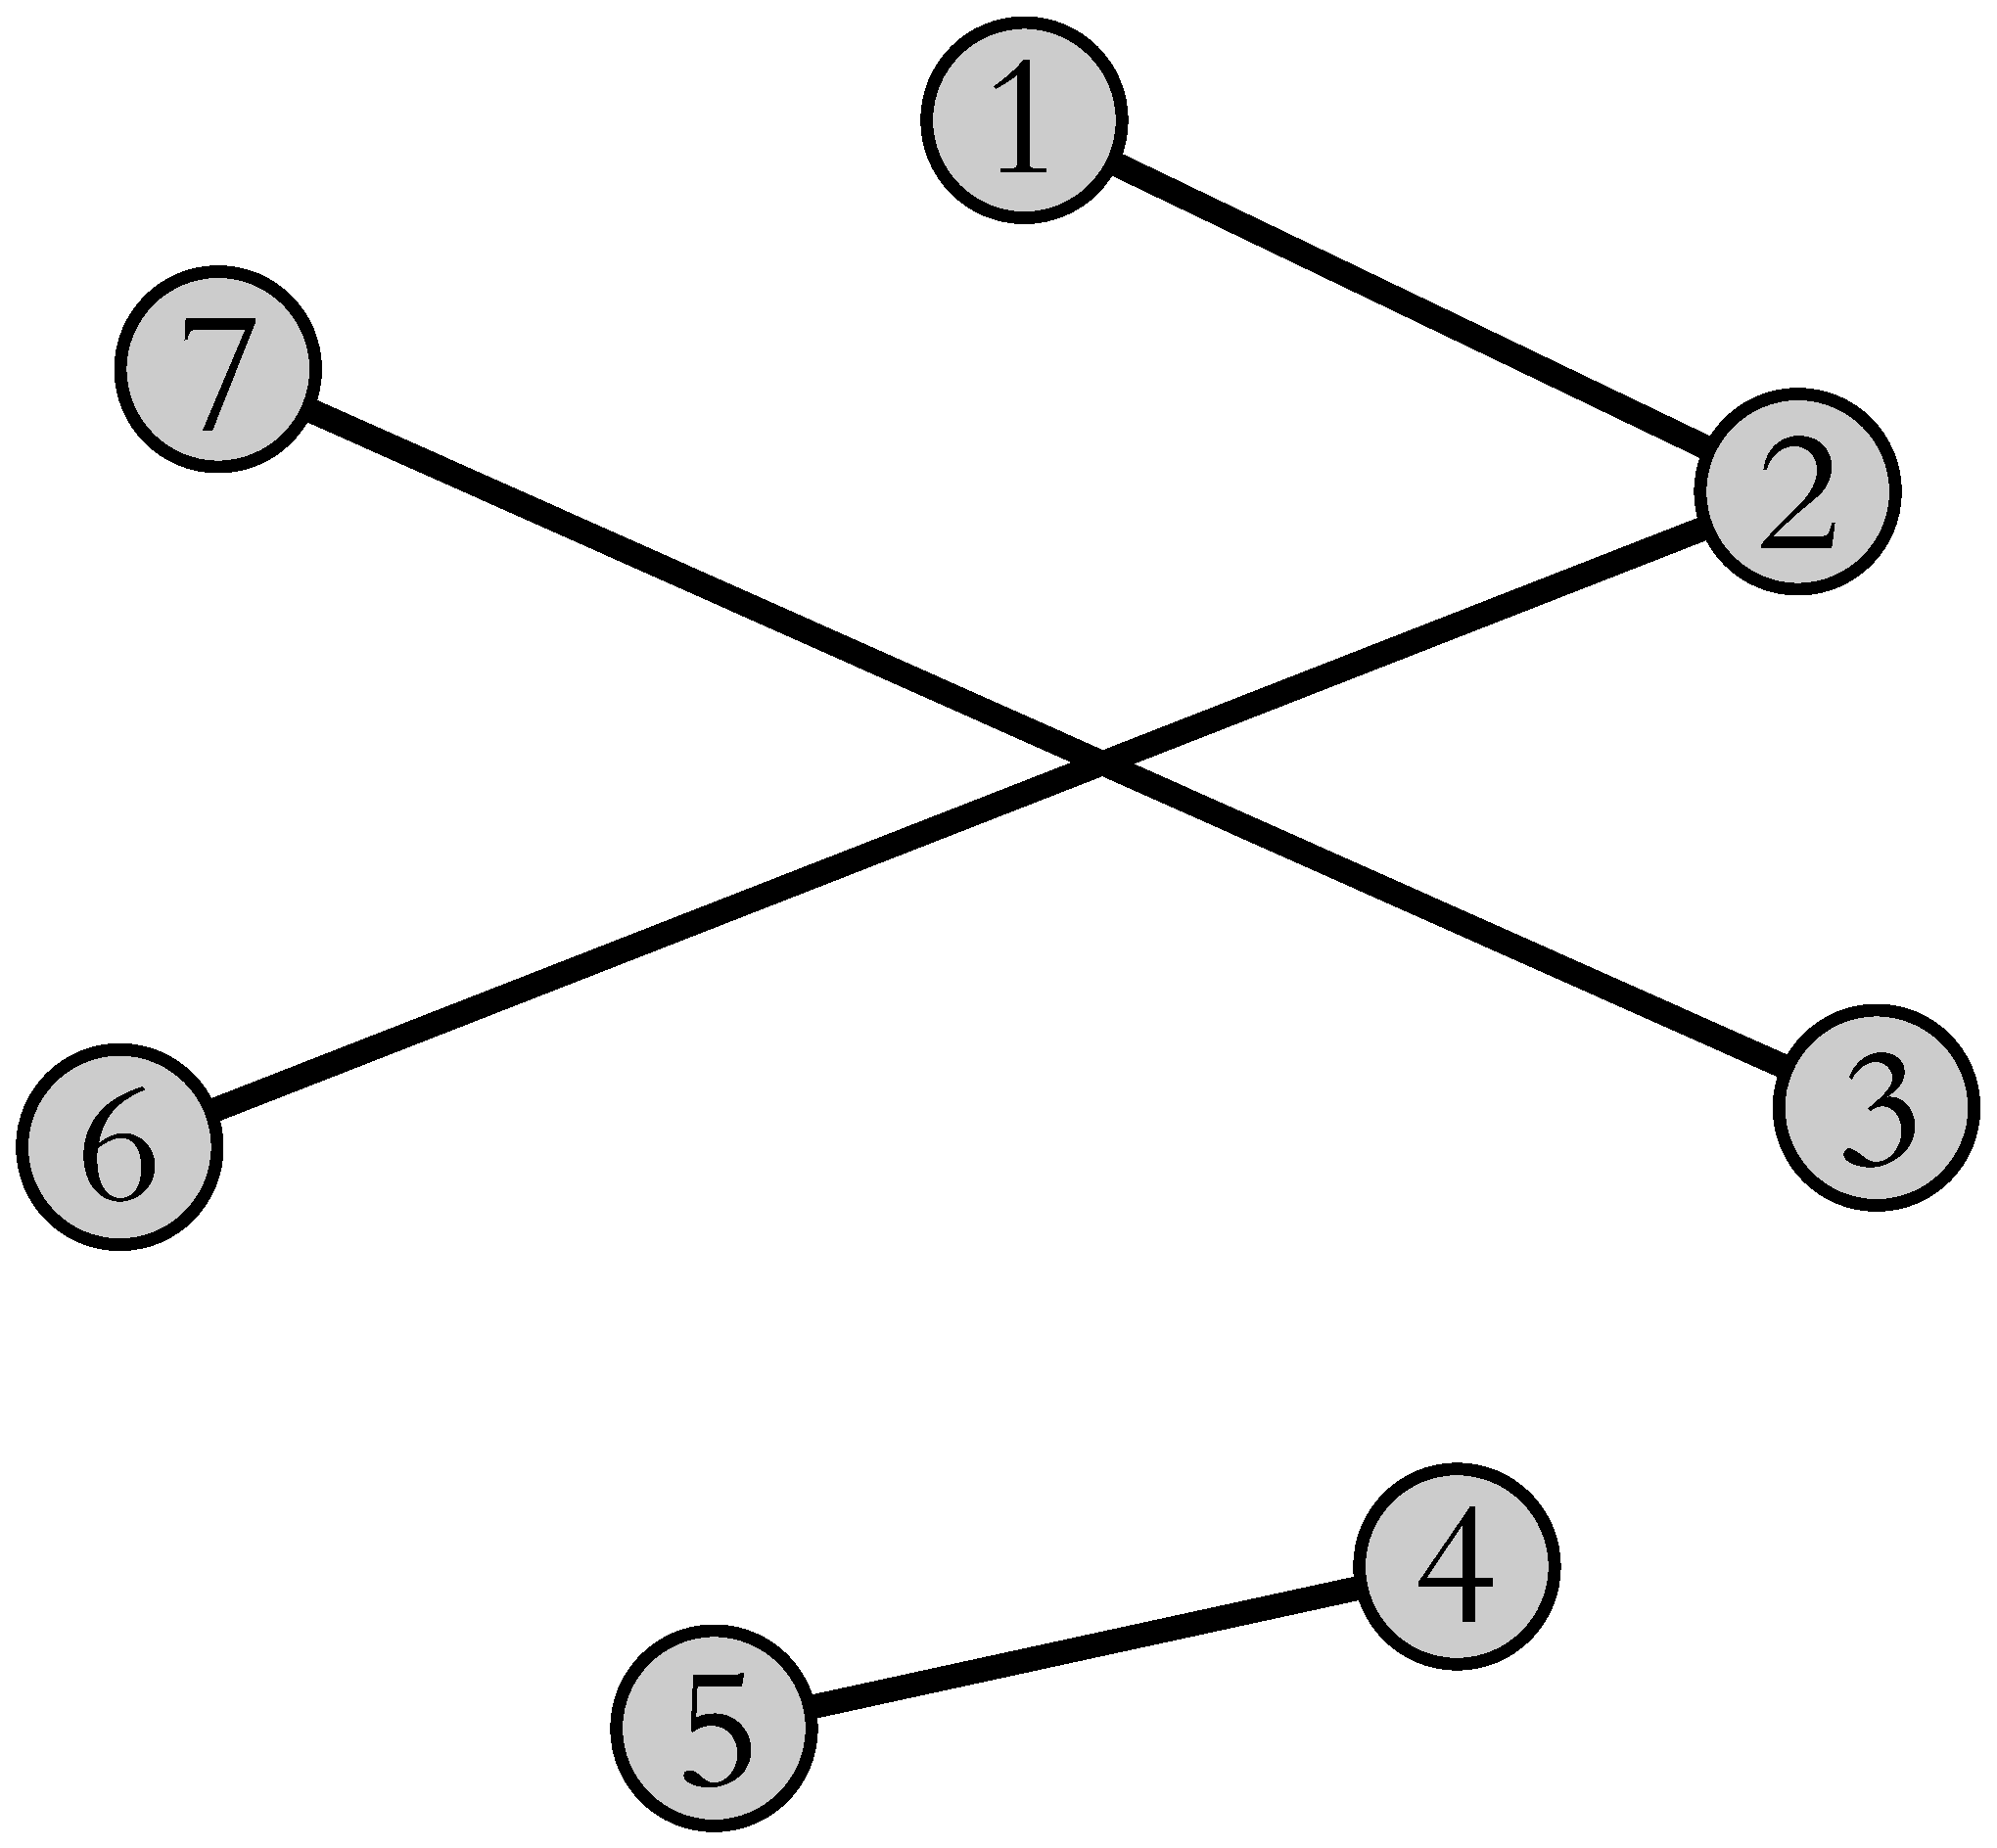
\includegraphics[width=60mm]{conflict_graph.eps}
\end{figure}

For first fit, we start from the first lightpath, assign the first free wavelength enumerating from $\lambda_1$ and move on the next lightpath. In most-used heuristics, the wavelength ordering is determined by the current usage of wavelengths in physical topology. The result of both algorithms is

{
\begin{table}[h]
\Large
\centering
\begin{tabular}{|c|c|c|c|}
\hline
Lightpath ID&Nodelist&First-fit&Most-used\\
\hline
1&E-A-C&$\lambda_1$&$\lambda_1$\\
\hline
2&A-C-G-F&$\lambda_2$&$\lambda_2$\\
\hline
3&F-E-C-D&$\lambda_1$&$\lambda_2$\\
\hline
4&B-D-C&$\lambda_1$&$\lambda_2$\\
\hline
5&A-B-D&$\lambda_2$&$\lambda_1$\\
\hline
6&C-G&$\lambda_1$&$\lambda_1$\\
\hline
7&C-D-B&$\lambda_2$&$\lambda_1$\\
\hline
\end{tabular}
\end{table}
}


\newpage

\Q

In topology pruning, we consider a wavelength and reduce the physical topology to those links with available (free) capacity on that wavelength. Two examples of pruning with respect to $\lambda_5$ and $\lambda_7$ are illustrated:
\begin{figure}[h]
\begin{subfigure}{0.49\textwidth}
\centering
\includegraphics[width=60mm]{net-wa-5.eps}
\caption{
Topology pruning with respect to $\lambda_5$
}
\end{subfigure}
\begin{subfigure}{0.49\textwidth}
\centering
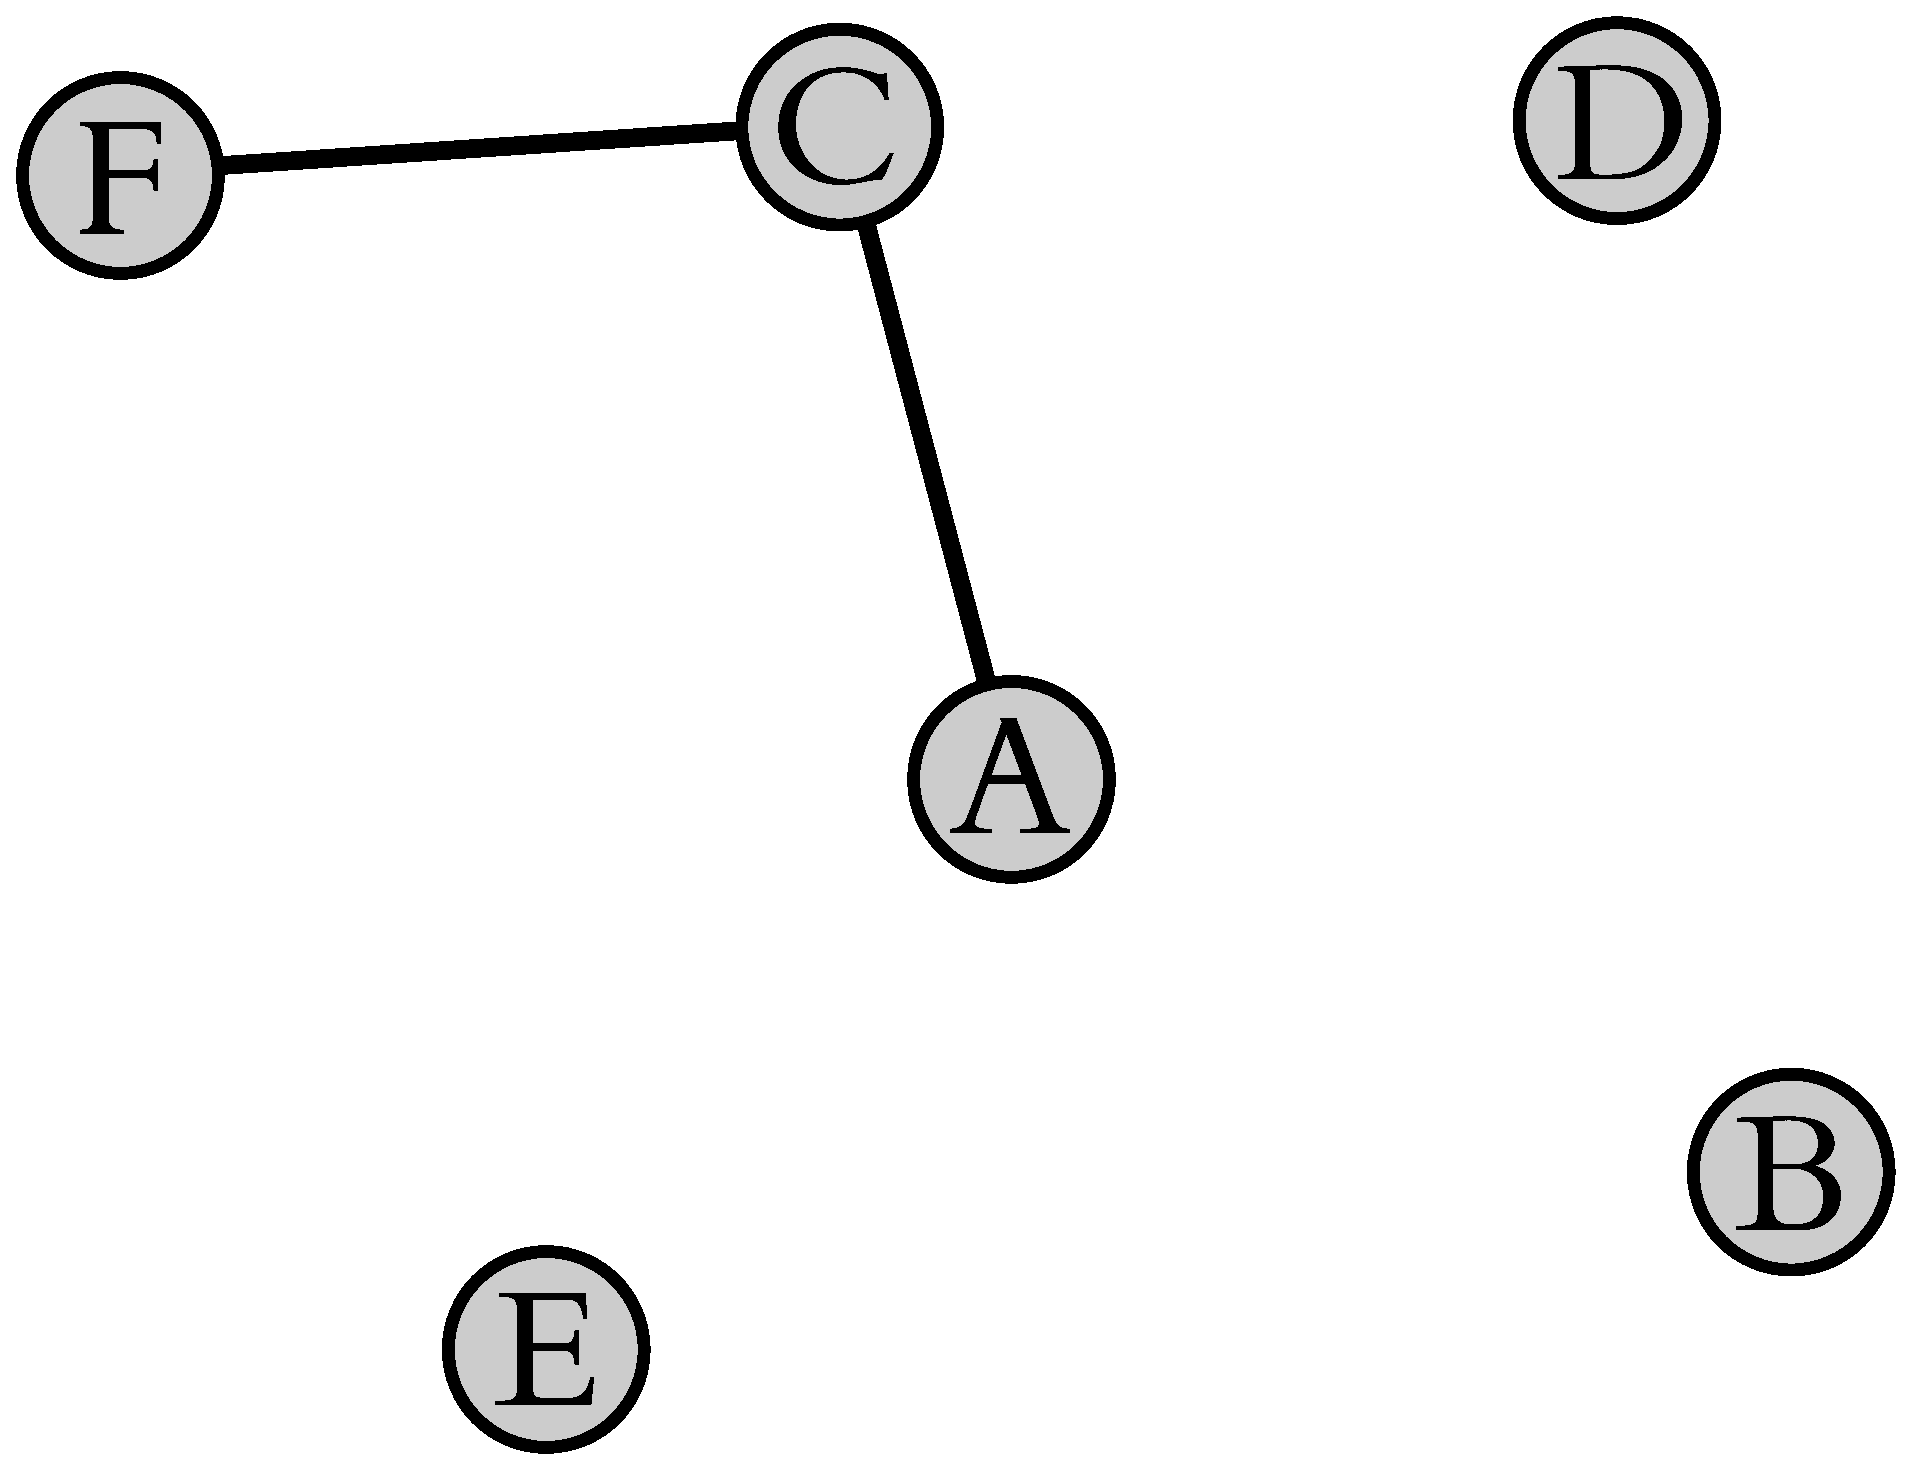
\includegraphics[width=60mm]{net-wa-7.eps}
\caption{
Topology pruning with respect to $\lambda_7$
}
\end{subfigure}
\caption{
Two examples of topology pruning
}
\end{figure}

\begin{enumerate}[label=\alph*-]
\item
Performing topology pruning with respect to all wavelengths, yields that the demand E-D can be routed over path E-A-D and wavelength $\lambda_5$, whereas F-B cannot be routed all optically.
\item
Performing regeneration in node A can solve the problem of blocking. As a consequence, the demand F-B can be routed over F-C-A-B where in the path section F-C-A, it is assigned $\lambda_7$ and in section A-B, it is assigned $\lambda_6$ through a wavelength conversion of $\lambda_7$ to $\lambda_6$.
\end{enumerate}
\begin{figure}[h]
\centering
\includegraphics[width=60mm]{net-wa-7-6.eps}
\caption{
Regeneration at node A for solving the blocked demand problem
}
\end{figure}
\end{document}